\documentclass{article}
\usepackage[utf8]{inputenc}
\usepackage[icelandic]{babel}
\usepackage[T1]{fontenc}
\usepackage{graphicx}
\usepackage{mathtools}
\usepackage{amsmath}
\usepackage{amssymb}
\usepackage{minted}


\graphicspath{ {./imgs} }
\title{Snake - Viðmótsforritun}
\author{ttb3@hi.is}
\date{\today}


\begin{document}
\maketitle


\section*{Gagnvirkniskröfur notenda}
\subsection*{1.}
\subsubsection*{Gagnvirkni}
    Notandi getur spilað Snake þar sem snákurinn getur borðað mat,stækkað og liðast, 
    snákurinn deyr svo ef hann snertir eitursnák eða klessir á sinn eiginn líkama.
\subsubsection*{Lýsing á verkefni} 
    Í fyrri útgáfu af Snake var aðeins hægt að lengjast en ekki liðast. 
    Með viðbættri liðunarhegðun þarf að breyta stjórnun á snáknum, 
    athuga þarf í hvaða átt snákurinn stefnir og koma í veg fyrir að hann snúi við.

\subsection*{2.}
\subsubsection*{Gagnvirkni}
Notandi getur skráð stigin sín niður ásamt þremur einkennisstöfum,
eins og í gömlum spilakössum.\footnote{Sjá mynd 2.1} Þessi stig eiga að geymast á milli leikja.

\subsubsection*{Lýsing á verkefni}
Hingað til hefur stigafjöldi verið vistaður sjálfkrafa og með enga vísun í notenda.
stigin voru aðeins til staðar frá því að leikurinn hafðist og þangað til að honum var lokað,
ekkert var geymt á milli keyrslna.

\subsection*{3.}
\subsubsection*{Gagnvirkni}
Notandi getur hefnt sín á eitursnákum, öðru hvoru er maturinn sem birtist 'sérstakur'
á þann hátt að þegar notandi borðar sérstaka matinn, 
getur hann ekki dáið og ef snákurinn rekst á eitursnák deyr eitursnákurinn.
Mjög svipuð pæling og stóru doppurnar í pac-man og stjörnur í super mario.
\footnote{Sjá myndir 3.1 og 3.2}

\subsubsection*{Lýsing á verkefni}

\section*{Myndir}
\begin{center}
    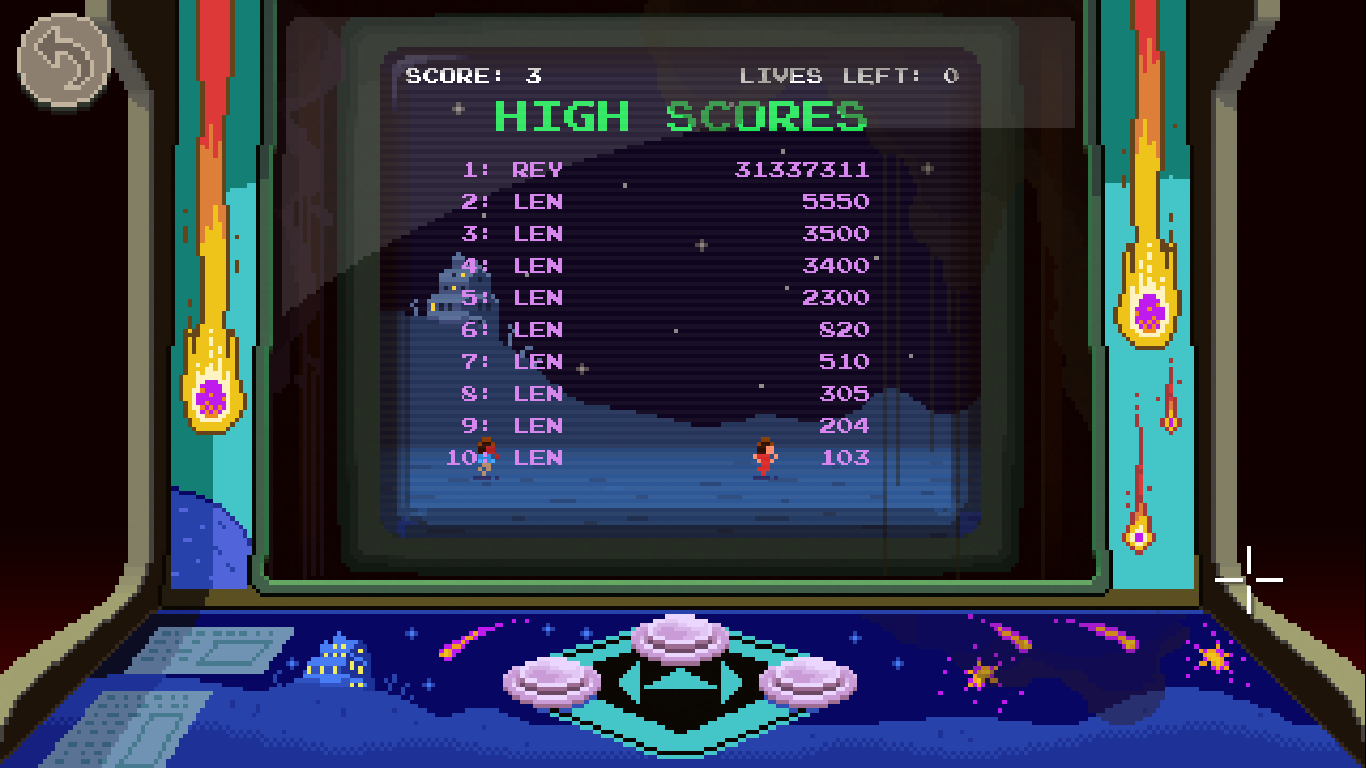
\includegraphics[scale=0.25]{imgs/highscore.png}
\end{center}
mynd 2.1

\begin{center}
    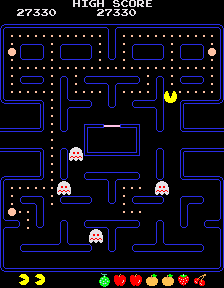
\includegraphics{imgs/pac-man.png}
\end{center}
mynd 3.1
\begin{center}
    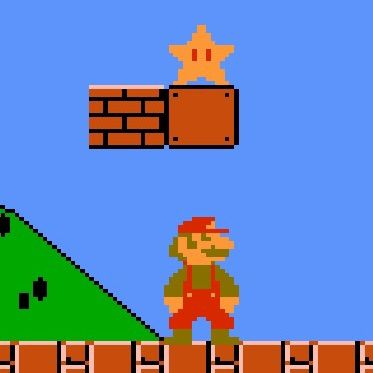
\includegraphics[scale=0.8]{imgs/mario.jpg}
\end{center}
mynd 3.2

\end{document}